\documentclass[]{book}
\usepackage{lmodern}
\usepackage{amssymb,amsmath}
\usepackage{ifxetex,ifluatex}
\usepackage{fixltx2e} % provides \textsubscript
\ifnum 0\ifxetex 1\fi\ifluatex 1\fi=0 % if pdftex
  \usepackage[T1]{fontenc}
  \usepackage[utf8]{inputenc}
\else % if luatex or xelatex
  \ifxetex
    \usepackage{mathspec}
  \else
    \usepackage{fontspec}
  \fi
  \defaultfontfeatures{Ligatures=TeX,Scale=MatchLowercase}
\fi
% use upquote if available, for straight quotes in verbatim environments
\IfFileExists{upquote.sty}{\usepackage{upquote}}{}
% use microtype if available
\IfFileExists{microtype.sty}{%
\usepackage{microtype}
\UseMicrotypeSet[protrusion]{basicmath} % disable protrusion for tt fonts
}{}
\usepackage[margin=1in]{geometry}
\usepackage{hyperref}
\hypersetup{unicode=true,
            pdftitle={Beginning Python For Programming},
            pdfauthor={Dan MacLean},
            pdfborder={0 0 0},
            breaklinks=true}
\urlstyle{same}  % don't use monospace font for urls
\usepackage{natbib}
\bibliographystyle{apalike}
\usepackage{color}
\usepackage{fancyvrb}
\newcommand{\VerbBar}{|}
\newcommand{\VERB}{\Verb[commandchars=\\\{\}]}
\DefineVerbatimEnvironment{Highlighting}{Verbatim}{commandchars=\\\{\}}
% Add ',fontsize=\small' for more characters per line
\usepackage{framed}
\definecolor{shadecolor}{RGB}{248,248,248}
\newenvironment{Shaded}{\begin{snugshade}}{\end{snugshade}}
\newcommand{\AlertTok}[1]{\textcolor[rgb]{0.94,0.16,0.16}{#1}}
\newcommand{\AnnotationTok}[1]{\textcolor[rgb]{0.56,0.35,0.01}{\textbf{\textit{#1}}}}
\newcommand{\AttributeTok}[1]{\textcolor[rgb]{0.77,0.63,0.00}{#1}}
\newcommand{\BaseNTok}[1]{\textcolor[rgb]{0.00,0.00,0.81}{#1}}
\newcommand{\BuiltInTok}[1]{#1}
\newcommand{\CharTok}[1]{\textcolor[rgb]{0.31,0.60,0.02}{#1}}
\newcommand{\CommentTok}[1]{\textcolor[rgb]{0.56,0.35,0.01}{\textit{#1}}}
\newcommand{\CommentVarTok}[1]{\textcolor[rgb]{0.56,0.35,0.01}{\textbf{\textit{#1}}}}
\newcommand{\ConstantTok}[1]{\textcolor[rgb]{0.00,0.00,0.00}{#1}}
\newcommand{\ControlFlowTok}[1]{\textcolor[rgb]{0.13,0.29,0.53}{\textbf{#1}}}
\newcommand{\DataTypeTok}[1]{\textcolor[rgb]{0.13,0.29,0.53}{#1}}
\newcommand{\DecValTok}[1]{\textcolor[rgb]{0.00,0.00,0.81}{#1}}
\newcommand{\DocumentationTok}[1]{\textcolor[rgb]{0.56,0.35,0.01}{\textbf{\textit{#1}}}}
\newcommand{\ErrorTok}[1]{\textcolor[rgb]{0.64,0.00,0.00}{\textbf{#1}}}
\newcommand{\ExtensionTok}[1]{#1}
\newcommand{\FloatTok}[1]{\textcolor[rgb]{0.00,0.00,0.81}{#1}}
\newcommand{\FunctionTok}[1]{\textcolor[rgb]{0.00,0.00,0.00}{#1}}
\newcommand{\ImportTok}[1]{#1}
\newcommand{\InformationTok}[1]{\textcolor[rgb]{0.56,0.35,0.01}{\textbf{\textit{#1}}}}
\newcommand{\KeywordTok}[1]{\textcolor[rgb]{0.13,0.29,0.53}{\textbf{#1}}}
\newcommand{\NormalTok}[1]{#1}
\newcommand{\OperatorTok}[1]{\textcolor[rgb]{0.81,0.36,0.00}{\textbf{#1}}}
\newcommand{\OtherTok}[1]{\textcolor[rgb]{0.56,0.35,0.01}{#1}}
\newcommand{\PreprocessorTok}[1]{\textcolor[rgb]{0.56,0.35,0.01}{\textit{#1}}}
\newcommand{\RegionMarkerTok}[1]{#1}
\newcommand{\SpecialCharTok}[1]{\textcolor[rgb]{0.00,0.00,0.00}{#1}}
\newcommand{\SpecialStringTok}[1]{\textcolor[rgb]{0.31,0.60,0.02}{#1}}
\newcommand{\StringTok}[1]{\textcolor[rgb]{0.31,0.60,0.02}{#1}}
\newcommand{\VariableTok}[1]{\textcolor[rgb]{0.00,0.00,0.00}{#1}}
\newcommand{\VerbatimStringTok}[1]{\textcolor[rgb]{0.31,0.60,0.02}{#1}}
\newcommand{\WarningTok}[1]{\textcolor[rgb]{0.56,0.35,0.01}{\textbf{\textit{#1}}}}
\usepackage{longtable,booktabs}
\usepackage{graphicx,grffile}
\makeatletter
\def\maxwidth{\ifdim\Gin@nat@width>\linewidth\linewidth\else\Gin@nat@width\fi}
\def\maxheight{\ifdim\Gin@nat@height>\textheight\textheight\else\Gin@nat@height\fi}
\makeatother
% Scale images if necessary, so that they will not overflow the page
% margins by default, and it is still possible to overwrite the defaults
% using explicit options in \includegraphics[width, height, ...]{}
\setkeys{Gin}{width=\maxwidth,height=\maxheight,keepaspectratio}
\IfFileExists{parskip.sty}{%
\usepackage{parskip}
}{% else
\setlength{\parindent}{0pt}
\setlength{\parskip}{6pt plus 2pt minus 1pt}
}
\setlength{\emergencystretch}{3em}  % prevent overfull lines
\providecommand{\tightlist}{%
  \setlength{\itemsep}{0pt}\setlength{\parskip}{0pt}}
\setcounter{secnumdepth}{5}
% Redefines (sub)paragraphs to behave more like sections
\ifx\paragraph\undefined\else
\let\oldparagraph\paragraph
\renewcommand{\paragraph}[1]{\oldparagraph{#1}\mbox{}}
\fi
\ifx\subparagraph\undefined\else
\let\oldsubparagraph\subparagraph
\renewcommand{\subparagraph}[1]{\oldsubparagraph{#1}\mbox{}}
\fi

%%% Use protect on footnotes to avoid problems with footnotes in titles
\let\rmarkdownfootnote\footnote%
\def\footnote{\protect\rmarkdownfootnote}

%%% Change title format to be more compact
\usepackage{titling}

% Create subtitle command for use in maketitle
\newcommand{\subtitle}[1]{
  \posttitle{
    \begin{center}\large#1\end{center}
    }
}

\setlength{\droptitle}{-2em}

  \title{Beginning Python For Programming}
    \pretitle{\vspace{\droptitle}\centering\huge}
  \posttitle{\par}
    \author{Dan MacLean}
    \preauthor{\centering\large\emph}
  \postauthor{\par}
      \predate{\centering\large\emph}
  \postdate{\par}
    \date{2018-12-14}

\usepackage{booktabs}

\usepackage{amsthm}
\newtheorem{theorem}{Theorem}[chapter]
\newtheorem{lemma}{Lemma}[chapter]
\theoremstyle{definition}
\newtheorem{definition}{Definition}[chapter]
\newtheorem{corollary}{Corollary}[chapter]
\newtheorem{proposition}{Proposition}[chapter]
\theoremstyle{definition}
\newtheorem{example}{Example}[chapter]
\theoremstyle{definition}
\newtheorem{exercise}{Exercise}[chapter]
\theoremstyle{remark}
\newtheorem*{remark}{Remark}
\newtheorem*{solution}{Solution}
\begin{document}
\maketitle

{
\setcounter{tocdepth}{1}
\tableofcontents
}
\begin{Shaded}
\begin{Highlighting}[]
\NormalTok{knitr}\OperatorTok{::}\NormalTok{opts_chunk}\OperatorTok{$}\KeywordTok{set}\NormalTok{(}\DataTypeTok{engine.path =} \KeywordTok{list}\NormalTok{(}
  \DataTypeTok{python =} \StringTok{'/Users/macleand/miniconda2/envs/programming_book/bin'}
\NormalTok{))}
\end{Highlighting}
\end{Shaded}

\hypertarget{prerequisites}{%
\chapter{Prerequisites}\label{prerequisites}}

No specific knowledge is assumed for this book, though you do need to
install some software.

\begin{enumerate}
\def\labelenumi{\arabic{enumi}.}
\tightlist
\item
  Python 3 via Anaconda
\item
  A reasonably recent web-browser
\item
  The \texttt{PyVCF} and \texttt{biopython} python packages
\item
  The file \href{assets/example.vcf}{example.vcf} and
  \href{assets/SRR020192.fastq.gz}{SRR020192.fastq.gz}
\end{enumerate}

\hypertarget{installing-python-3-with-anaconda}{%
\section{Installing Python 3 with
Anaconda}\label{installing-python-3-with-anaconda}}

Follow this link and install Python \emph{3.x} for your operating
system. \url{https://www.anaconda.com/distribution/}

\hypertarget{note-for-macos-users}{%
\subsection{Note for macOS users}\label{note-for-macos-users}}

Accept all of the defaults during installation

Here is a video tutorial
\url{https://www.youtube.com/watch?v=TcSAln46u9U}

\hypertarget{note-for-windows-users}{%
\subsection{Note for Windows users}\label{note-for-windows-users}}

Install Python 3 using all of the defaults for installation except make
sure to check \textbf{Add Anaconda to my PATH environment variable}.

Here is a video tutorial
\url{https://www.youtube.com/watch?v=xxQ0mzZ8UvA}

\hypertarget{note-for-linux-users}{%
\subsection{Note for Linux Users}\label{note-for-linux-users}}

You'll need to be able to use the command-line to install with Anaconda.
If you aren't comfortable with this, ask for assistance from the local
support team.

\begin{enumerate}
\def\labelenumi{\arabic{enumi}.}
\tightlist
\item
  Open \href{}{https://www.anaconda.com/download/\#linux} with your web
  browser.
\item
  Download the Python 3 installer for Linux.
\item
  Open a terminal window. 4.Type \texttt{bash\ Anaconda3-}and then press
  Tab. The name of the file you just downloaded should appear. If it
  does not, navigate to the folder where you downloaded the file, for
  example with: \texttt{cd\ Downloads}. Then, try again.
\item
  Press \texttt{enter}. You will follow the text-only prompts. To move
  through the text, press the \texttt{spacebar}.
\item
  Type \texttt{yes} and press \texttt{enter} to approve the license.
\item
  Press \texttt{enter} to approve the default location for the files.
\item
  Type \texttt{yes} and press \texttt{enter} to prepend Anaconda to your
  \texttt{PATH} (this makes the Anaconda distribution the default
  Python).
\item
  Close the terminal window.
\end{enumerate}

\hypertarget{starting-a-jupyter-notebook}{%
\section{Starting a Jupyter
Notebook}\label{starting-a-jupyter-notebook}}

\hypertarget{macos}{%
\subsection{macOS}\label{macos}}

\begin{enumerate}
\def\labelenumi{\arabic{enumi}.}
\tightlist
\item
  Start the \texttt{Terminal} application in
  \texttt{Applications\ -\textgreater{}\ Utilities}
\item
  Type \texttt{jupyter\ notebook}, it should start in your web browser
\end{enumerate}

\hypertarget{windows}{%
\subsection{Windows}\label{windows}}

\begin{enumerate}
\def\labelenumi{\arabic{enumi}.}
\tightlist
\item
  From the Start menu, search for and open \texttt{Anaconda\ 3} or
  \texttt{Jupyter\ Notebook}. You should be able to start a notebook
  directly by clicking the \texttt{Jupyter\ Notebook} icon.
\end{enumerate}

\hypertarget{linux}{%
\subsection{Linux}\label{linux}}

\begin{enumerate}
\def\labelenumi{\arabic{enumi}.}
\tightlist
\item
  Open the terminal application. It is \emph{usually} in the task bar or
  dock
\item
  Type \texttt{jupyter\ notebook}, it should start in your web browser
\end{enumerate}

\hypertarget{installing-python-packages-with-conda}{%
\section{\texorpdfstring{Installing Python Packages with
\texttt{conda}}{Installing Python Packages with conda}}\label{installing-python-packages-with-conda}}

You can use \texttt{conda} to install new Python packages with
\texttt{conda\ install\ \textless{}package\_name\textgreater{}}. You can
install the required packages with

\begin{verbatim}
conda install PyVCF
conda install biopython
\end{verbatim}

Accept all defaults when the system asks a question.

\hypertarget{motivation}{%
\chapter{Motivation}\label{motivation}}

Programming is a pretty weird skill. It boils down to shouting at a
computer to make it do stuff for you. So why would you want to learn to
do it? Well, there are plenty of reasons, some good and some bad. Some
good ones that apply to working in biology and bioinformatics are
time-saving, turning your computer from a limited `appliance' to a
general `power tool' for your research and because it's a skill that can
help you develop a more precise, disciplined and abstract way of
thinking.

The main obstacle that most people encounter when learning to program is
the surprisingly wide range of facts that you need to know in order to
achieve something. This can make it

The aim of this course is to introduce you to just enough of these facts
and tricks to enable you to do useful stuff with programming. The things
you'll learn here will seem quite abstract and disconnected at first but
hopefully by the end of the course you'll be able to string them
together to make something useful - and understand what's going on.

In this course, we'll use Python 3 as our programming language - it's a
widely used very powerful but (all things considered) user-friendly
language that suits beginners and experts alike (well, as well as any
programming language can suit human users).

We'll use the bare-bones of Python 3, it is a very broad language with a
lot of functionality, a lot of it in optional packages that you can
install at will. We'll only touch the surface of what you can do - but
what we learn will be foundation enough to build pretty much anything
on.

\hypertarget{data}{%
\chapter{Working with Data}\label{data}}

\begin{enumerate}
\def\labelenumi{\arabic{enumi}.}
\tightlist
\item
  Questions:
\end{enumerate}

\begin{itemize}
\tightlist
\item
  How do I deal with data in Python?
\end{itemize}

\begin{enumerate}
\def\labelenumi{\arabic{enumi}.}
\setcounter{enumi}{1}
\tightlist
\item
  Objectives:
\end{enumerate}

\begin{itemize}
\tightlist
\item
  Defining variables and using them in functions
\item
  Using simple data objects: strings and numbers
\item
  Using package functions and object methods
\end{itemize}

\begin{enumerate}
\def\labelenumi{\arabic{enumi}.}
\setcounter{enumi}{2}
\tightlist
\item
  Keypoints:
\end{enumerate}

\begin{itemize}
\tightlist
\item
  variables are handy names for data objects
\item
  variables are used in functions
\item
  functions can be stored in packages
\item
  methods available depend on the object we're talking about
\end{itemize}

In any Python program we will have some data and some objective to
achieve - something to do with that data. Python provides many data
types and many ways of working with that data.

Let's see the simplest example of this, let's take a string (a text
carrying data type) and use it in a function.

\begin{Shaded}
\begin{Highlighting}[]
\BuiltInTok{print}\NormalTok{(}\StringTok{"Hello, world!"}\NormalTok{)}
\end{Highlighting}
\end{Shaded}

\begin{verbatim}
## Hello, world!
\end{verbatim}

In this example is the text \texttt{"Hello,\ World!"}, is being given to
the \texttt{print()} function. Functions are bits of code that do stuff
to data. The \texttt{print()} function just prints the data you pass it
to the screen. We pass data to functions by putting the data in the
brackets after the function name.

\texttt{print()} just tries to print the data you give it to the screen.

\hypertarget{using-variables-as-names-for-data}{%
\section{Using variables as names for
data}\label{using-variables-as-names-for-data}}

We don't usually use data as directly as this. Instead we use a name
that refers to a piece of data - a variable. Variables are just names
that represent a bit of data. It's called a variable because the data
the variable is associated with can change. We assign a name to data by
using the assignment symbol the \texttt{=} sign. The data associated
with a variable can be changed by re-assignment. allowing us to reuse
the name.

We can use variables as if they were the data they point to

\begin{Shaded}
\begin{Highlighting}[]
\NormalTok{x }\OperatorTok{=} \StringTok{"Hello, world!"}
\BuiltInTok{print}\NormalTok{(x)}
\end{Highlighting}
\end{Shaded}

\begin{verbatim}
## Hello, world!
\end{verbatim}

\begin{Shaded}
\begin{Highlighting}[]
\NormalTok{x }\OperatorTok{=} \DecValTok{100}
\BuiltInTok{print}\NormalTok{(x)}
\end{Highlighting}
\end{Shaded}

\begin{verbatim}
## 100
\end{verbatim}

And variables are independent of one another, actions on one don't
affect another

\begin{Shaded}
\begin{Highlighting}[]
\NormalTok{weight_kg }\OperatorTok{=} \DecValTok{65}
\NormalTok{weight_pounds }\OperatorTok{=} \FloatTok{2.2} \OperatorTok{*}\NormalTok{ weight_kg}
\BuiltInTok{print}\NormalTok{(weight_kg)}
\end{Highlighting}
\end{Shaded}

\begin{verbatim}
## 65
\end{verbatim}

\begin{Shaded}
\begin{Highlighting}[]
\BuiltInTok{print}\NormalTok{(weight_pounds)}
\end{Highlighting}
\end{Shaded}

\begin{verbatim}
## 143.0
\end{verbatim}

\hypertarget{functions-from-different-places}{%
\section{Functions from different
places}\label{functions-from-different-places}}

We can work on data objects in Python using three different types of
function

\begin{itemize}
\tightlist
\item
  Object Methods
\item
  Built-In Functions and Operators
\item
  Package Functions
\end{itemize}

\hypertarget{built-in-functions-and-operators}{%
\subsection{Built-In Functions and
Operators}\label{built-in-functions-and-operators}}

Python has some functions that can be called directly from anywhere in a
program. These are listed here
\href{}{https://docs.python.org/3.3/library/functions.html}. We've
already seen \texttt{print()} `and there are some common ones we'll come
across later. You can spot a built-in function because it has a
single-word name followed by brackets.

Related to built-in functions are operators. The things you'll use most
are the mathematical operators that work as you would expect from your
knowledge of maths. So they include things like,
\texttt{+\ ,\ -,\ *,\ /} etc.

\begin{Shaded}
\begin{Highlighting}[]
\BuiltInTok{print}\NormalTok{(}\DecValTok{1} \OperatorTok{+} \DecValTok{1}\NormalTok{)}
\end{Highlighting}
\end{Shaded}

\begin{verbatim}
## 2
\end{verbatim}

\begin{Shaded}
\begin{Highlighting}[]
\BuiltInTok{print}\NormalTok{(}\DecValTok{2} \OperatorTok{*} \DecValTok{2}\NormalTok{)}
\end{Highlighting}
\end{Shaded}

\begin{verbatim}
## 4
\end{verbatim}

\begin{Shaded}
\begin{Highlighting}[]
\BuiltInTok{print}\NormalTok{(}\DecValTok{3} \OperatorTok{-} \DecValTok{3}\NormalTok{)}
\end{Highlighting}
\end{Shaded}

\begin{verbatim}
## 0
\end{verbatim}

\begin{Shaded}
\begin{Highlighting}[]
\BuiltInTok{print}\NormalTok{(}\DecValTok{4} \OperatorTok{/} \DecValTok{4}\NormalTok{)}
\end{Highlighting}
\end{Shaded}

\begin{verbatim}
## 1.0
\end{verbatim}

Some operators change what they do depending on the things you ask them
to operate on. For instance, we can add strings?!

\begin{Shaded}
\begin{Highlighting}[]
\BuiltInTok{print}\NormalTok{( }\StringTok{"Hello"} \OperatorTok{+} \StringTok{"World!"}\NormalTok{)}
\end{Highlighting}
\end{Shaded}

\begin{verbatim}
## HelloWorld!
\end{verbatim}

\hypertarget{package-methods}{%
\subsection{Package Methods}\label{package-methods}}

Another source of functions is external packages - extensions to Python
for use in particular problem domains. We can load in a package using
\texttt{import}. Let's import the \texttt{numpy} numerical Python
package that provides functions for doing fast, large scale numerical
analysis.

\begin{Shaded}
\begin{Highlighting}[]
\ImportTok{import}\NormalTok{ numpy}
\end{Highlighting}
\end{Shaded}

We can access the functions in this package by using the package name
and the dot (\texttt{.}) syntax and the function name. Let's call the
numpy function \texttt{arange()} which gives us a list of numbers.

\begin{Shaded}
\begin{Highlighting}[]
\NormalTok{numbers }\OperatorTok{=}\NormalTok{ numpy.arange(}\DecValTok{10}\NormalTok{)}
\BuiltInTok{print}\NormalTok{( numbers )}
\end{Highlighting}
\end{Shaded}

\begin{verbatim}
## [0 1 2 3 4 5 6 7 8 9]
\end{verbatim}

\hypertarget{object-methods}{%
\subsection{Object Methods}\label{object-methods}}

Python's data are represented in the computer in things called objects.
An object is basically a bit of data with some functions attached. So
that each piece of data comes with the code to manipulate it. These
attached functions are called \texttt{methods}.

We access data's methods using the \texttt{.} syntax, so you have
\texttt{variable\_name.method()}, read this as you telling the variable
to do \texttt{method()} to itself, so a text containing variable
\texttt{x} used with \texttt{.capitalize()} comes to

\begin{Shaded}
\begin{Highlighting}[]
\NormalTok{x }\OperatorTok{=} \StringTok{"hello, world!"}
\BuiltInTok{print}\NormalTok{( x.capitalize() )}
\end{Highlighting}
\end{Shaded}

\begin{verbatim}
## Hello, world!
\end{verbatim}

This does mean that the methods are closely tied to the data. Look what
happens when we try to use \texttt{.capitalize()} on a number

\begin{Shaded}
\begin{Highlighting}[]
\NormalTok{y }\OperatorTok{=} \DecValTok{100}
\BuiltInTok{print}\NormalTok{( y.capitalize() )}
\end{Highlighting}
\end{Shaded}

\begin{verbatim}
Error in py_run_string_impl(code, local, convert) : 
  AttributeError: 'int' object has no attribute 'capitalize'
\end{verbatim}

Python just throws an error. Basically this error is saying that
\texttt{int} (integer, a number object ) doesn't have a method called
\texttt{capitalize}.

We need to know what methods an object has before we can work on them.
We can find this by reading the documentation for the object type. And
Python will give us the type with the \texttt{type()} function

\begin{Shaded}
\begin{Highlighting}[]
\BuiltInTok{print}\NormalTok{( }\BuiltInTok{type}\NormalTok{(x) )}
\end{Highlighting}
\end{Shaded}

\begin{verbatim}
## <class 'str'>
\end{verbatim}

We can see that \texttt{x} contains a \texttt{str} - a string. The
easiest place to find the Python documentation is online. Googling
\texttt{Python\ 3\ str} shows us this page
\href{}{https://docs.python.org/3/library/stdtypes.html\#text-sequence-type-str},
which shows us all the String methods. This works well for finding all
methods for objects of other types.

\hypertarget{objects-and-types-in-python}{%
\section{Objects and types in
Python}\label{objects-and-types-in-python}}

Python knows many types of object, most things are an object of some
type. Three common object types are:

\begin{itemize}
\tightlist
\item
  strings
\item
  integer numbers
\item
  floating point numbers
\end{itemize}

\hypertarget{string-objects}{%
\subsection{String Objects}\label{string-objects}}

The term 'strings` is computer jargon for text data, usually a single
lump of text data treated as a whole.

And to create a strings we simply have to add single or double quotes
around some text, for example:

\begin{Shaded}
\begin{Highlighting}[]
\NormalTok{weight_kg_text }\OperatorTok{=} \StringTok{'weight in kilograms'}
\end{Highlighting}
\end{Shaded}

Having actual numbers in there doesn't make a string a number type - the
following is still a string - it just happens to be made up of number
like characters. Let's see what happens if we try and treat it like a
number.

\begin{Shaded}
\begin{Highlighting}[]
\NormalTok{phone_number }\OperatorTok{=} \StringTok{"01818118181"}
\BuiltInTok{print}\NormalTok{( phone_number }\OperatorTok{*} \DecValTok{2}\NormalTok{ )}
\end{Highlighting}
\end{Shaded}

\begin{verbatim}
## 0181811818101818118181
\end{verbatim}

Here the \texttt{*} operator has modified itself to work on a string and
repeated the string!

\hypertarget{indexing-a-string-slicing}{%
\subsubsection{Indexing a string
(Slicing)}\label{indexing-a-string-slicing}}

We can access a single character in a string using indexing - basically
asking for a character at a position. The syntax uses the square
brackets.

\begin{Shaded}
\begin{Highlighting}[]
\BuiltInTok{print}\NormalTok{( phone_number[}\DecValTok{2}\NormalTok{] )}
\end{Highlighting}
\end{Shaded}

\begin{verbatim}
## 8
\end{verbatim}

Note that using the index \texttt{{[}2{]}} gives us the \emph{third}
character - computer languages tend to count from \texttt{0}.

We can get a longer subsection of a string using indexing as well - this
is a technique that accesses a part of the data given a start and end
point along the string.

\begin{Shaded}
\begin{Highlighting}[]
\NormalTok{dialling_code }\OperatorTok{=}\NormalTok{ phone_number[}\DecValTok{0}\NormalTok{:}\DecValTok{3}\NormalTok{]}
\BuiltInTok{print}\NormalTok{(dialling_code)}
\end{Highlighting}
\end{Shaded}

\begin{verbatim}
## 018
\end{verbatim}

We just use the square brackets to indicate the start and stop points of
the slice we want to extract, literally \texttt{{[}start:end{]}}. The
\texttt{start} here is \texttt{0} meaning the first character, the
\texttt{end} here is \texttt{3}, but it means
\texttt{up\ to\ but\ not\ including\ the\ end}.

\begin{Shaded}
\begin{Highlighting}[]
\BuiltInTok{print}\NormalTok{( dialling_code )}
\end{Highlighting}
\end{Shaded}

\begin{verbatim}
## 018
\end{verbatim}

That's why we only get the first three characters from the string and
not 4 ie \texttt{0,1,2,3}. The way to remember this is that the length
of the resulting slice is \texttt{end} - \texttt{start}.

There are many string operations and methods, you can see them in the
documentation at
\href{}{https://docs.python.org/3/library/stdtypes.html\#textseq}

\hypertarget{number-objects}{%
\subsection{Number Objects}\label{number-objects}}

Numbers in Python come in two types, whole numbers (called integers) and
numbers with a decimal part (called floating point numbers).

In the example above, variable \texttt{weight\_kg} has an integer value
of \texttt{65}. To create a variable with a floating point value, we can
execute:

\begin{Shaded}
\begin{Highlighting}[]
\NormalTok{weight_kg }\OperatorTok{=} \FloatTok{65.0}
\end{Highlighting}
\end{Shaded}

The difference is important. Operations with integers return only
integers.

\begin{Shaded}
\begin{Highlighting}[]
\BuiltInTok{print}\NormalTok{( }\DecValTok{10} \OperatorTok{/} \DecValTok{3}\NormalTok{ )}
\end{Highlighting}
\end{Shaded}

\begin{verbatim}
## 3.3333333333333335
\end{verbatim}

Operations with floating points return floating points

\begin{Shaded}
\begin{Highlighting}[]
\BuiltInTok{print}\NormalTok{( }\FloatTok{10.0} \OperatorTok{/} \FloatTok{3.0}\NormalTok{ )}
\end{Highlighting}
\end{Shaded}

\begin{verbatim}
## 3.3333333333333335
\end{verbatim}

\begin{Shaded}
\begin{Highlighting}[]
\BuiltInTok{print}\NormalTok{( }\DecValTok{10} \OperatorTok{/} \FloatTok{3.0}\NormalTok{ )}
\end{Highlighting}
\end{Shaded}

\begin{verbatim}
## 3.3333333333333335
\end{verbatim}

\begin{Shaded}
\begin{Highlighting}[]
\BuiltInTok{print}\NormalTok{( }\FloatTok{10.0} \OperatorTok{/} \DecValTok{3}\NormalTok{)}
\end{Highlighting}
\end{Shaded}

\begin{verbatim}
## 3.3333333333333335
\end{verbatim}

You can convert type explicitly using the \texttt{int()} and
\texttt{float()} functions.

\begin{Shaded}
\begin{Highlighting}[]
\BuiltInTok{print}\NormalTok{( }\BuiltInTok{float}\NormalTok{(}\DecValTok{10}\NormalTok{) }\OperatorTok{/} \DecValTok{3}\NormalTok{ )}
\end{Highlighting}
\end{Shaded}

\begin{verbatim}
## 3.3333333333333335
\end{verbatim}

\begin{Shaded}
\begin{Highlighting}[]
\BuiltInTok{print}\NormalTok{( }\BuiltInTok{int}\NormalTok{( }\FloatTok{10.0} \OperatorTok{/} \FloatTok{3.0}\NormalTok{ ) )}
\end{Highlighting}
\end{Shaded}

\begin{verbatim}
## 3
\end{verbatim}

\hypertarget{quiz}{%
\section{Quiz}\label{quiz}}

\begin{enumerate}
\def\labelenumi{\arabic{enumi}.}
\tightlist
\item
  What values do the variables \texttt{mass} and \texttt{age} have after
  each statement in the following program? Test your answers by
  executing the commands.
\end{enumerate}

\begin{verbatim}
 mass = 47.5
 age = 122
 mass = mass * 2.0
 age = age - 20
\end{verbatim}

\begin{enumerate}
\def\labelenumi{\arabic{enumi}.}
\setcounter{enumi}{1}
\tightlist
\item
  What does the following program print out?
\end{enumerate}

\begin{verbatim}
 first, second = 'Grace', 'Hopper'
 third, fourth = second, first
 print(third, fourth)
\end{verbatim}

\begin{enumerate}
\def\labelenumi{\arabic{enumi}.}
\setcounter{enumi}{2}
\tightlist
\item
  Recall that a section of string is called a
  \href{\%7B\%7B\%20page.root\%20\%7D\%7D/reference/\#slice}{slice}.
\end{enumerate}

\begin{verbatim}
 element = 'oxygen'
 print('first three characters:', element[0:3])
 print('last three characters:', element[3:6])
\end{verbatim}

\begin{itemize}
\tightlist
\item
  What is the value of \texttt{element{[}:4{]}}?
\item
  What about \texttt{element{[}4:{]}}?
\item
  Or \texttt{element{[}:{]}}?
\item
  What is \texttt{element{[}-1{]}}?
\item
  What is \texttt{element{[}-2{]}}?
\item
  Given those answers, explain what \texttt{element{[}1:-1{]}} does.
\end{itemize}

\begin{enumerate}
\def\labelenumi{\arabic{enumi}.}
\setcounter{enumi}{3}
\tightlist
\item
  Fix the capitalisation in \texttt{messy\_string}
\end{enumerate}

\begin{verbatim}
messy_string = "OH mY, ThESE LEtters Are ALL OVER The PLace!"
\end{verbatim}

Hint: Think about standardising the letters by e.g making all one case,
then fixing the capitalization from there.

\begin{enumerate}
\def\labelenumi{\arabic{enumi}.}
\setcounter{enumi}{4}
\tightlist
\item
  Check out the \texttt{math} package.
  \href{}{https://docs.python.org/3/library/math.html} and
  \texttt{import} it.
\end{enumerate}

\begin{itemize}
\tightlist
\item
  What is the arc sine of \texttt{-1}, \texttt{0}, \texttt{1} in
  radians?
\item
  How many degrees in \(\arcsin(-1)\) radians?
\end{itemize}

\hypertarget{data-structures}{%
\chapter{Data Structures}\label{data-structures}}

\begin{enumerate}
\def\labelenumi{\arabic{enumi}.}
\tightlist
\item
  Questions:
\end{enumerate}

\begin{itemize}
\tightlist
\item
  How do I arrange and process lots of data in Python?
\end{itemize}

\begin{enumerate}
\def\labelenumi{\arabic{enumi}.}
\setcounter{enumi}{1}
\tightlist
\item
  Objectives:
\end{enumerate}

\begin{itemize}
\tightlist
\item
  Create and work with \texttt{lists} and \texttt{dicts}
\item
  Using loops and conditionals to make decisions
\end{itemize}

\begin{enumerate}
\def\labelenumi{\arabic{enumi}.}
\setcounter{enumi}{2}
\tightlist
\item
  Keypoints:
\end{enumerate}

\begin{itemize}
\tightlist
\item
  variables are handy names for data objects
\item
  variables are used in functions
\item
  functions can be stored in packages
\item
  methods available depend on the object we're talking about
\end{itemize}

\hypertarget{lists}{%
\section{Lists}\label{lists}}

Like most programming languages Python has some built in data structures
that we can use.

Data structures are collection types that group lots of data into a
single object and make working with lots of data easier. The simplest
data structure is a \texttt{list}. We can create a list simply by
enclosing our data in square brackets.

\begin{Shaded}
\begin{Highlighting}[]
\NormalTok{my_list }\OperatorTok{=}\NormalTok{ [}\DecValTok{1}\NormalTok{,}\DecValTok{3}\NormalTok{,}\DecValTok{5}\NormalTok{,}\DecValTok{7}\NormalTok{]}
\BuiltInTok{print}\NormalTok{( my_list )}
\end{Highlighting}
\end{Shaded}

\begin{verbatim}
## [1, 3, 5, 7]
\end{verbatim}

More often, though, we'll get a \texttt{list} as the result of a
function. Recall the \texttt{numpy} function we used earlier.

\begin{Shaded}
\begin{Highlighting}[]
\ImportTok{import}\NormalTok{ numpy}
\NormalTok{numbers }\OperatorTok{=}\NormalTok{ numpy.arange(}\DecValTok{15}\NormalTok{)}
\BuiltInTok{print}\NormalTok{( numbers )}
\end{Highlighting}
\end{Shaded}

\begin{verbatim}
## [ 0  1  2  3  4  5  6  7  8  9 10 11 12 13 14]
\end{verbatim}

\hypertarget{list-use}{%
\subsection{List use}\label{list-use}}

Lists can mix up any sort of data type,

\begin{Shaded}
\begin{Highlighting}[]
\NormalTok{numbers_and_letters }\OperatorTok{=}\NormalTok{ [}\DecValTok{1}\NormalTok{,}\DecValTok{2}\NormalTok{, }\StringTok{'three'}\NormalTok{, }\StringTok{'IV'}\NormalTok{, }\FloatTok{5.0}\NormalTok{ ]}
\BuiltInTok{print}\NormalTok{( numbers_and_letters )}
\end{Highlighting}
\end{Shaded}

\begin{verbatim}
## [1, 2, 'three', 'IV', 5.0]
\end{verbatim}

including other lists.

\begin{Shaded}
\begin{Highlighting}[]
\NormalTok{list_of_lists }\OperatorTok{=}\NormalTok{ [ [}\DecValTok{1}\NormalTok{,}\DecValTok{2}\NormalTok{,}\DecValTok{3}\NormalTok{], [}\StringTok{"a"}\NormalTok{,}\StringTok{"b"}\NormalTok{,}\StringTok{"c"}\NormalTok{] ]}
\BuiltInTok{print}\NormalTok{( list_of_lists )}
\end{Highlighting}
\end{Shaded}

\begin{verbatim}
## [[1, 2, 3], ['a', 'b', 'c']]
\end{verbatim}

List elements can be accessed using indexing, like with strings.

\begin{Shaded}
\begin{Highlighting}[]
\BuiltInTok{print}\NormalTok{( numbers_and_letters[}\DecValTok{0}\NormalTok{] )}
\end{Highlighting}
\end{Shaded}

\begin{verbatim}
## 1
\end{verbatim}

\begin{Shaded}
\begin{Highlighting}[]
\BuiltInTok{print}\NormalTok{( numbers_and_letters[}\DecValTok{2}\NormalTok{:}\DecValTok{3}\NormalTok{] )}
\end{Highlighting}
\end{Shaded}

\begin{verbatim}
## ['three']
\end{verbatim}

Indexing an element returns the whole element - so if that element
happens to be a list itself - you get a whole list back

\begin{Shaded}
\begin{Highlighting}[]
\BuiltInTok{print}\NormalTok{( list_of_lists[}\DecValTok{1}\NormalTok{] )}
\end{Highlighting}
\end{Shaded}

\begin{verbatim}
## ['a', 'b', 'c']
\end{verbatim}

To get at a single element you must use double square brackets.

\begin{Shaded}
\begin{Highlighting}[]
\BuiltInTok{print}\NormalTok{( list_of_lists[}\DecValTok{0}\NormalTok{][}\DecValTok{1}\NormalTok{] )}
\end{Highlighting}
\end{Shaded}

\begin{verbatim}
## 2
\end{verbatim}

\begin{Shaded}
\begin{Highlighting}[]
\BuiltInTok{print}\NormalTok{( list_of_lists[}\DecValTok{1}\NormalTok{][}\DecValTok{0}\NormalTok{] )}
\end{Highlighting}
\end{Shaded}

\begin{verbatim}
## a
\end{verbatim}

\hypertarget{dictionaries}{%
\section{Dictionaries}\label{dictionaries}}

Another very common data structure is a dictionary. A dictionary is a
data structure that has many unique \texttt{keys}, each of which refers
to a bit of other data called a \texttt{value}. We can construct them
using the curly brackets and the \texttt{key/value} pairs

\begin{Shaded}
\begin{Highlighting}[]
\NormalTok{my_dict }\OperatorTok{=}\NormalTok{ \{}
  \StringTok{"key1"}\NormalTok{ : }\StringTok{"value1"}\NormalTok{,}
  \StringTok{"key2"}\NormalTok{ : }\StringTok{"value2"}
\NormalTok{\}}
\BuiltInTok{print}\NormalTok{( my_dict )}
\end{Highlighting}
\end{Shaded}

\begin{verbatim}
## {'key1': 'value1', 'key2': 'value2'}
\end{verbatim}

Note the order in the dictionary isn't preserved. We can use the square
brackets to get a single value, but as a dictionary has no order or
index, we must use the key.

\begin{Shaded}
\begin{Highlighting}[]
\BuiltInTok{print}\NormalTok{( my_dict[}\StringTok{"key1"}\NormalTok{] )}
\end{Highlighting}
\end{Shaded}

\begin{verbatim}
## value1
\end{verbatim}

Dictionaries are useful when you want to ask for a bit of data by some
name, rather than by its position in a list.

Dictionaries can hold anything in their values. But keys are restricted
to particular datatypes. Strings and numbers are good keys, lists are
not allowed.

\begin{Shaded}
\begin{Highlighting}[]
\BuiltInTok{print}\NormalTok{( \{ [}\StringTok{"list_key"}\NormalTok{, }\DecValTok{1}\NormalTok{, }\DecValTok{2}\NormalTok{] : [}\StringTok{"some data"}\NormalTok{]  \} )}
\end{Highlighting}
\end{Shaded}

\begin{verbatim}
Traceback (most recent call last):
  File "<stdin>", line 1, in <module>
TypeError: unhashable type: 'list'
\end{verbatim}

\hypertarget{quiz-1}{%
\section{Quiz}\label{quiz-1}}

\begin{enumerate}
\def\labelenumi{\arabic{enumi}.}
\tightlist
\item
  Given the list below, use slicing to access only the last four
  entries.
\end{enumerate}

\begin{Shaded}
\begin{Highlighting}[]
\NormalTok{list_for_slicing }\OperatorTok{=}\NormalTok{ [[}\StringTok{"fluorine"}\NormalTok{, }\StringTok{"F"}\NormalTok{], }
\NormalTok{                    [}\StringTok{"chlorine"}\NormalTok{, }\StringTok{"Cl"}\NormalTok{], }
\NormalTok{                    [}\StringTok{"bromine"}\NormalTok{, }\StringTok{"Br"}\NormalTok{], }
\NormalTok{                    [}\StringTok{"iodine"}\NormalTok{, }\StringTok{"I"}\NormalTok{], }
\NormalTok{                    [}\StringTok{"astatine"}\NormalTok{, }\StringTok{"At"}\NormalTok{]]}
\end{Highlighting}
\end{Shaded}

\begin{enumerate}
\def\labelenumi{\arabic{enumi}.}
\setcounter{enumi}{1}
\tightlist
\item
  Can you work out how to correct the wrong data in the dictionary
  below? Try to think of a way that \emph{doesn't} involve re-writing
  the whole dictionary. Hint: can you assign straight to a key?
\end{enumerate}

\begin{Shaded}
\begin{Highlighting}[]
\NormalTok{seasons }\OperatorTok{=}\NormalTok{ \{}
  \StringTok{'spring'}\NormalTok{ : [}\StringTok{'mar'}\NormalTok{, }\StringTok{'apr'}\NormalTok{, }\StringTok{'may'}\NormalTok{ ],}
  \StringTok{'autumn'}\NormalTok{ : [}\StringTok{'jun'}\NormalTok{, }\StringTok{'jul'}\NormalTok{, }\StringTok{'aug'}\NormalTok{],}
  \StringTok{'winter'}\NormalTok{ : [}\StringTok{'dec'}\NormalTok{, }\StringTok{'jan'}\NormalTok{, }\StringTok{'feb'}\NormalTok{]}
\NormalTok{\}}
\end{Highlighting}
\end{Shaded}

\begin{enumerate}
\def\labelenumi{\arabic{enumi}.}
\setcounter{enumi}{2}
\tightlist
\item
  Add in the missing season.
\end{enumerate}

\hypertarget{making-choices-and-controlling-program-flow}{%
\chapter{Making Choices and Controlling Program
Flow}\label{making-choices-and-controlling-program-flow}}

How can we use Python to automatically recognize differences in data
such that it can change what code is run depending on the data and take
a different action for each? In this chapter, we'll learn how to write
code that runs only when certain conditions are true.

\hypertarget{conditionals}{%
\section{Conditionals}\label{conditionals}}

We can ask Python to take different actions, depending on a condition,
with an \texttt{if} statement:

\begin{Shaded}
\begin{Highlighting}[]
\NormalTok{num }\OperatorTok{=} \DecValTok{37}
\ControlFlowTok{if}\NormalTok{ num }\OperatorTok{>} \DecValTok{100}\NormalTok{:}
    \BuiltInTok{print}\NormalTok{(}\StringTok{'greater'}\NormalTok{)}
\ControlFlowTok{else}\NormalTok{:}
    \BuiltInTok{print}\NormalTok{(}\StringTok{'not greater'}\NormalTok{)}
\end{Highlighting}
\end{Shaded}

\begin{verbatim}
## not greater
\end{verbatim}

The second line of this code uses the keyword \texttt{if} to tell Python
that we want to make a choice. If the test that follows the \texttt{if}
statement is true, the body of the \texttt{if} (i.e., the lines indented
underneath it) are executed. If the test is false, the body of the
\texttt{else} is executed instead. Only one or the other is ever
executed:

The diagram below shows how this choice is being made.

\begin{figure}
\centering
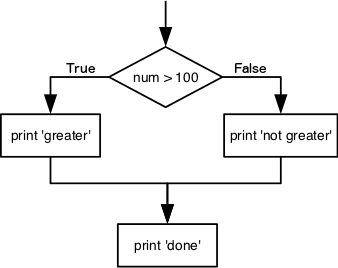
\includegraphics{assets/python-flowchart-conditional.png}
\caption{Executing a Conditional}
\end{figure}

Conditional statements don't have to include an \texttt{else}. If there
isn't one, Python simply does nothing if the test is false:

\begin{Shaded}
\begin{Highlighting}[]
\NormalTok{num }\OperatorTok{=} \DecValTok{53}
\BuiltInTok{print}\NormalTok{(}\StringTok{'before conditional...'}\NormalTok{)}
\end{Highlighting}
\end{Shaded}

\begin{verbatim}
## before conditional...
\end{verbatim}

\begin{Shaded}
\begin{Highlighting}[]
\ControlFlowTok{if}\NormalTok{ num }\OperatorTok{>} \DecValTok{100}\NormalTok{:}
    \BuiltInTok{print}\NormalTok{(num,}\StringTok{' is greater than 100'}\NormalTok{)}
\BuiltInTok{print}\NormalTok{(}\StringTok{'...after conditional'}\NormalTok{)}
\end{Highlighting}
\end{Shaded}

\begin{verbatim}
## ...after conditional
\end{verbatim}

We can also chain several tests together using \texttt{elif}, which is
short for ``else if''. The following Python code uses \texttt{elif} to
print the sign of a number.

\begin{Shaded}
\begin{Highlighting}[]
\NormalTok{num }\OperatorTok{=} \DecValTok{-3}
\ControlFlowTok{if}\NormalTok{ num }\OperatorTok{>} \DecValTok{0}\NormalTok{:}
    \BuiltInTok{print}\NormalTok{(num, }\StringTok{'is positive'}\NormalTok{)}
\ControlFlowTok{elif}\NormalTok{ num }\OperatorTok{==} \DecValTok{0}\NormalTok{:}
    \BuiltInTok{print}\NormalTok{(num, }\StringTok{'is zero'}\NormalTok{)}
\ControlFlowTok{else}\NormalTok{:}
    \BuiltInTok{print}\NormalTok{(num, }\StringTok{'is negative'}\NormalTok{)}
\end{Highlighting}
\end{Shaded}

\begin{verbatim}
## -3 is negative
\end{verbatim}

Note that the \texttt{if} and \texttt{elif} bits are mutually exclusive.
Only one of them ever gets executed.

\hypertarget{testing-equality}{%
\subsection{Testing equality}\label{testing-equality}}

Note that to test for equality we use a double equals sign \texttt{==}
rather than a single equals sign \texttt{=} which is already used to
assign values.

\hypertarget{logical-operators}{%
\section{Logical operators}\label{logical-operators}}

Python has all the standard logical operators that let us combine tests.
Most commonly there is \texttt{and} and \texttt{or}. \texttt{and} is
only true if both parts are true:

\begin{Shaded}
\begin{Highlighting}[]
\ControlFlowTok{if}\NormalTok{ (}\DecValTok{1} \OperatorTok{>} \DecValTok{0}\NormalTok{) }\KeywordTok{and}\NormalTok{ (}\OperatorTok{-}\DecValTok{1} \OperatorTok{>} \DecValTok{0}\NormalTok{):}
    \BuiltInTok{print}\NormalTok{(}\StringTok{'both parts are true'}\NormalTok{)}
\ControlFlowTok{else}\NormalTok{:}
    \BuiltInTok{print}\NormalTok{(}\StringTok{'at least one part is false'}\NormalTok{)}
\end{Highlighting}
\end{Shaded}

\begin{verbatim}
## at least one part is false
\end{verbatim}

while \texttt{or} is true if at least one part is true:

\begin{Shaded}
\begin{Highlighting}[]
\ControlFlowTok{if}\NormalTok{ (}\DecValTok{1} \OperatorTok{<} \DecValTok{0}\NormalTok{) }\KeywordTok{or}\NormalTok{ (}\OperatorTok{-}\DecValTok{1} \OperatorTok{<} \DecValTok{0}\NormalTok{):}
    \BuiltInTok{print}\NormalTok{(}\StringTok{'at least one test is true'}\NormalTok{)}
\end{Highlighting}
\end{Shaded}

\begin{verbatim}
## at least one test is true
\end{verbatim}

\hypertarget{what-is-true-and-what-is-false}{%
\subsection{What is True and what is
False}\label{what-is-true-and-what-is-false}}

True and \texttt{False} \texttt{True} and \texttt{False} are special
words in Python called \texttt{booleans}, which represent truth values.
A statement such as \texttt{1\ \textless{}\ 0} returns the value
\texttt{False}, while \texttt{-1\ \textless{}\ 0} returns the value
\texttt{True}.

\texttt{True} and \texttt{False} booleans are not the only values in
Python that are true and false. In fact, \emph{any} value can be used in
an \texttt{if} or \texttt{elif}. After reading and running the code
below, explain what the rule is for which values are considered true and
which are considered false.

\begin{Shaded}
\begin{Highlighting}[]
\ControlFlowTok{if} \StringTok{''}\NormalTok{:}
    \BuiltInTok{print}\NormalTok{(}\StringTok{'empty string is true'}\NormalTok{)}
\ControlFlowTok{if} \StringTok{'word'}\NormalTok{:}
    \BuiltInTok{print}\NormalTok{(}\StringTok{'word is true'}\NormalTok{)}
\end{Highlighting}
\end{Shaded}

\begin{verbatim}
## word is true
\end{verbatim}

\begin{Shaded}
\begin{Highlighting}[]
\ControlFlowTok{if}\NormalTok{ []:}
    \BuiltInTok{print}\NormalTok{(}\StringTok{'empty list is true'}\NormalTok{)}
\ControlFlowTok{if}\NormalTok{ [}\DecValTok{1}\NormalTok{, }\DecValTok{2}\NormalTok{, }\DecValTok{3}\NormalTok{]:}
    \BuiltInTok{print}\NormalTok{(}\StringTok{'non-empty list is true'}\NormalTok{)}
\end{Highlighting}
\end{Shaded}

\begin{verbatim}
## non-empty list is true
\end{verbatim}

\begin{Shaded}
\begin{Highlighting}[]
\ControlFlowTok{if} \DecValTok{0}\NormalTok{:}
     \BuiltInTok{print}\NormalTok{(}\StringTok{'zero is true'}\NormalTok{)}
\ControlFlowTok{if} \DecValTok{1}\NormalTok{:}
    \BuiltInTok{print}\NormalTok{(}\StringTok{'one is true'}\NormalTok{)}
\end{Highlighting}
\end{Shaded}

\begin{verbatim}
## one is true
\end{verbatim}

\hypertarget{thats-not-not-what-i-meant}{%
\section{That's Not Not What I Meant}\label{thats-not-not-what-i-meant}}

Sometimes it is useful to check whether some condition is not true. The
Boolean operator \texttt{not} can do this explicitly. After reading and
running the code below, write some \texttt{if} statements that use
\texttt{not} to test the rule that you formulated in the previous
challenge.

\begin{Shaded}
\begin{Highlighting}[]
\ControlFlowTok{if} \KeywordTok{not} \StringTok{''}\NormalTok{:}
    \BuiltInTok{print}\NormalTok{(}\StringTok{'empty string is not true'}\NormalTok{)}
\end{Highlighting}
\end{Shaded}

\begin{verbatim}
## empty string is not true
\end{verbatim}

\begin{Shaded}
\begin{Highlighting}[]
\ControlFlowTok{if} \KeywordTok{not} \StringTok{'word'}\NormalTok{:}
    \BuiltInTok{print}\NormalTok{(}\StringTok{'word is not true'}\NormalTok{)}
\ControlFlowTok{if} \KeywordTok{not} \KeywordTok{not} \VariableTok{True}\NormalTok{:}
    \BuiltInTok{print}\NormalTok{(}\StringTok{'not not True is true'}\NormalTok{)}
\end{Highlighting}
\end{Shaded}

\begin{verbatim}
## not not True is true
\end{verbatim}

\hypertarget{quiz-2}{%
\section{Quiz}\label{quiz-2}}

\begin{enumerate}
\def\labelenumi{\arabic{enumi}.}
\tightlist
\item
  Consider this code:
\end{enumerate}

\begin{Shaded}
\begin{Highlighting}[]
\ControlFlowTok{if} \DecValTok{4} \OperatorTok{>} \DecValTok{5}\NormalTok{:}
    \BuiltInTok{print}\NormalTok{(}\StringTok{'A'}\NormalTok{)}
\ControlFlowTok{elif} \DecValTok{4} \OperatorTok{==} \DecValTok{5}\NormalTok{:}
    \BuiltInTok{print}\NormalTok{(}\StringTok{'B'}\NormalTok{)}
\ControlFlowTok{elif} \DecValTok{4} \OperatorTok{<} \DecValTok{5}\NormalTok{:}
    \BuiltInTok{print}\NormalTok{(}\StringTok{'C'}\NormalTok{)}
\end{Highlighting}
\end{Shaded}

Which of the following would be printed if you were to run this code?
Why did you pick this answer?

\begin{itemize}
\tightlist
\item
  A
\item
  B
\item
  C
\item
  B and C
\end{itemize}

\begin{enumerate}
\def\labelenumi{\arabic{enumi}.}
\setcounter{enumi}{1}
\tightlist
\item
  Consider this code:
\end{enumerate}

\begin{Shaded}
\begin{Highlighting}[]
\ControlFlowTok{if} \DecValTok{4} \OperatorTok{>} \DecValTok{5}\NormalTok{:}
    \BuiltInTok{print}\NormalTok{(}\StringTok{'A'}\NormalTok{)}
\ControlFlowTok{if} \DecValTok{4} \OperatorTok{<=} \DecValTok{5}\NormalTok{:}
    \BuiltInTok{print}\NormalTok{(}\StringTok{'B'}\NormalTok{)}
\ControlFlowTok{if} \DecValTok{4} \OperatorTok{<} \DecValTok{5}\NormalTok{:}
    \BuiltInTok{print}\NormalTok{(}\StringTok{'C'}\NormalTok{)}
\end{Highlighting}
\end{Shaded}

Which of the following would be printed if you were to run this code?
Why did you pick this answer?

\begin{itemize}
\tightlist
\item
  A
\item
  B
\item
  C
\item
  B and C
\end{itemize}

\begin{enumerate}
\def\labelenumi{\arabic{enumi}.}
\setcounter{enumi}{2}
\tightlist
\item
  Consider this code:
\end{enumerate}

\begin{Shaded}
\begin{Highlighting}[]
\ControlFlowTok{if} \DecValTok{4} \OperatorTok{>} \DecValTok{5}\NormalTok{:}
    \BuiltInTok{print}\NormalTok{(}\StringTok{'A'}\NormalTok{)}
\ControlFlowTok{elif} \DecValTok{4} \OperatorTok{<=} \DecValTok{5}\NormalTok{:}
    \BuiltInTok{print}\NormalTok{(}\StringTok{'B'}\NormalTok{)}
\ControlFlowTok{elif} \DecValTok{4} \OperatorTok{<} \DecValTok{5}\NormalTok{:}
    \BuiltInTok{print}\NormalTok{(}\StringTok{'C'}\NormalTok{)}
\end{Highlighting}
\end{Shaded}

Which of the following would be printed if you were to run this code?
Why did you pick this answer?

\begin{itemize}
\tightlist
\item
  A
\item
  B
\item
  C
\item
  B and C
\end{itemize}

\hypertarget{repeating-actions-with-loops}{%
\chapter{Repeating actions with
Loops}\label{repeating-actions-with-loops}}

To do that, we'll have to teach the computer how to repeat things.

An example task that we might want to repeat is printing each character
in a word on a line of its own.

We can access a character in a string using its index. For example, we
can get the first character of the word
\texttt{\textquotesingle{}lead\textquotesingle{}}, by using
\texttt{word{[}0{]}}. One way to print each character is to use four
\texttt{print} statements:

\begin{Shaded}
\begin{Highlighting}[]
\NormalTok{word }\OperatorTok{=} \StringTok{'lead'}
\BuiltInTok{print}\NormalTok{(word[}\DecValTok{0}\NormalTok{])}
\end{Highlighting}
\end{Shaded}

\begin{verbatim}
## l
\end{verbatim}

\begin{Shaded}
\begin{Highlighting}[]
\BuiltInTok{print}\NormalTok{(word[}\DecValTok{1}\NormalTok{])}
\end{Highlighting}
\end{Shaded}

\begin{verbatim}
## e
\end{verbatim}

\begin{Shaded}
\begin{Highlighting}[]
\BuiltInTok{print}\NormalTok{(word[}\DecValTok{2}\NormalTok{])}
\end{Highlighting}
\end{Shaded}

\begin{verbatim}
## a
\end{verbatim}

\begin{Shaded}
\begin{Highlighting}[]
\BuiltInTok{print}\NormalTok{(word[}\DecValTok{3}\NormalTok{])}
\end{Highlighting}
\end{Shaded}

\begin{verbatim}
## d
\end{verbatim}

This is a bad approach for two reasons:

\begin{enumerate}
\def\labelenumi{\arabic{enumi}.}
\tightlist
\item
  It doesn't scale: if we want to print the characters in a string
  that's hundreds of letters long, we'd be better off just typing them
  in.
\item
  It's fragile: if we give it a longer string, it only prints part of
  the data, and if we give it a shorter one,it produces an error because
  we're asking for characters that don't exist.
\end{enumerate}

\begin{Shaded}
\begin{Highlighting}[]
\NormalTok{word }\OperatorTok{=} \StringTok{'tin'}
\BuiltInTok{print}\NormalTok{(word[}\DecValTok{0}\NormalTok{])}
\BuiltInTok{print}\NormalTok{(word[}\DecValTok{1}\NormalTok{])}
\BuiltInTok{print}\NormalTok{(word[}\DecValTok{2}\NormalTok{])}
\BuiltInTok{print}\NormalTok{(word[}\DecValTok{3}\NormalTok{])}
\end{Highlighting}
\end{Shaded}

\begin{verbatim}
---------------------------------------------------------------------------
IndexError                                Traceback (most recent call last)
<ipython-input-3-7974b6cdaf14> in <module>()
      3 print(word[1])
      4 print(word[2])
----> 5 print(word[3])

IndexError: string index out of range
\end{verbatim}

\hypertarget{for-loops}{%
\section{For Loops}\label{for-loops}}

Instead we can use a loop - a construct that moves through a collection
of data taking one bit at a time. Here's a loop in action

\begin{Shaded}
\begin{Highlighting}[]
\NormalTok{word }\OperatorTok{=} \StringTok{'lead'}
\ControlFlowTok{for}\NormalTok{ char }\KeywordTok{in}\NormalTok{ word:}
    \BuiltInTok{print}\NormalTok{(char)}
\end{Highlighting}
\end{Shaded}

\begin{verbatim}
## l
## e
## a
## d
\end{verbatim}

This is shorter, certainly shorter than something that prints every
character in a hundred-letter string and more robust as well. See how
the same code works if we change the length of the word

\begin{Shaded}
\begin{Highlighting}[]
\NormalTok{word }\OperatorTok{=} \StringTok{'oxygen'}
\ControlFlowTok{for}\NormalTok{ char }\KeywordTok{in}\NormalTok{ word:}
    \BuiltInTok{print}\NormalTok{(char)}
\end{Highlighting}
\end{Shaded}

\begin{verbatim}
## o
## x
## y
## g
## e
## n
\end{verbatim}

The improved version uses a for loop to repeat code in this case
\texttt{print()}, once for each thing in a sequence. The general form of
a loop is:

Using the oxygen example above, the loop might look like this:

\begin{figure}
\centering
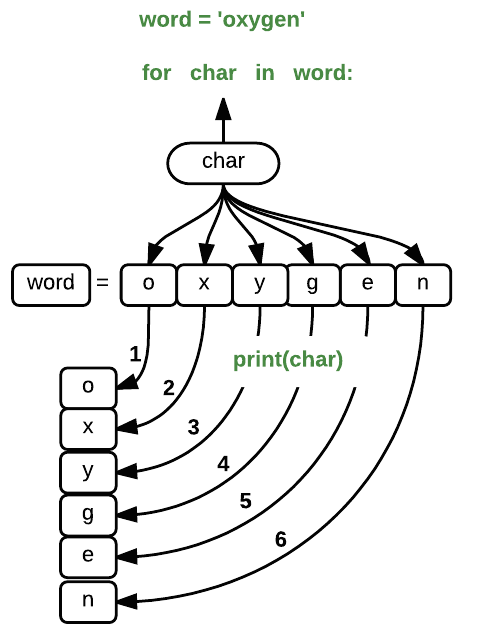
\includegraphics{assets/loops_image.png}
\caption{loop\_image}
\end{figure}

where each character (\texttt{char}) in the variable \texttt{word} is
looped through and printed one character after another. The numbers in
the diagram denote which loop cycle the character was printed in (1
being the first loop, and 6 being the final loop).

We can call the loop variable anything we like, but there must be a
colon at the end of the line starting the loop, and we must indent
anything we want to run inside the loop. Unlike many other languages,
there is no command to signify the end of the loop body (e.g.
\texttt{end\ for}); what is indented after the \texttt{for} statement
belongs to the loop.

\hypertarget{choosing-loop-variable-names}{%
\subsection{Choosing loop variable
names}\label{choosing-loop-variable-names}}

In the example above, the loop variable was given the name \texttt{char}
as a mnemonic; it is short for `character'. We can choose any name we
want for variables. We might just as easily have chosen the name
\texttt{banana} for the loop variable, as long as we use the same name
when we invoke the variable inside

\begin{Shaded}
\begin{Highlighting}[]
\NormalTok{word }\OperatorTok{=} \StringTok{'oxygen'}
\ControlFlowTok{for}\NormalTok{ banana }\KeywordTok{in}\NormalTok{ word:}
    \BuiltInTok{print}\NormalTok{(banana)}
\end{Highlighting}
\end{Shaded}

\begin{verbatim}
## o
## x
## y
## g
## e
## n
\end{verbatim}

It is a good idea to choose variable names that are meaningful,
otherwise it would be more difficult to understand what the loop is
doing.

Here's another loop that repeatedly updates a variable:

\begin{Shaded}
\begin{Highlighting}[]
\NormalTok{length }\OperatorTok{=} \DecValTok{0}
\ControlFlowTok{for}\NormalTok{ vowel }\KeywordTok{in} \StringTok{'aeiou'}\NormalTok{:}
\NormalTok{    length }\OperatorTok{=}\NormalTok{ length }\OperatorTok{+} \DecValTok{1}
\BuiltInTok{print}\NormalTok{(}\StringTok{'There are'}\NormalTok{, length, }\StringTok{'vowels'}\NormalTok{)}
\end{Highlighting}
\end{Shaded}

\begin{verbatim}
## There are 5 vowels
\end{verbatim}

It's worth tracing the execution of this little program step by
step.Since there are five characters in
\texttt{\textquotesingle{}aeiou\textquotesingle{}},the statement on line
3 will be executed five times.The first time around,\texttt{length} is
zero (the value assigned to it on line 1) and \texttt{vowel} is
\texttt{\textquotesingle{}a\textquotesingle{}}. The statement adds 1 to
the old value of \texttt{length}, producing 1, and updates
\texttt{length} to refer to that new value.

The next time around,\texttt{vowel} is
\texttt{\textquotesingle{}e\textquotesingle{}} and \texttt{length} is 1,
so \texttt{length} is updated to be 2. After three more updates,
\texttt{length} is 5; since there is nothing left in
\texttt{\textquotesingle{}aeiou\textquotesingle{}} for Python to
process, the loop finishes and the \texttt{print} statement on line 4
tells us our final answer.

\hypertarget{loop-variable-lifespan}{%
\subsection{Loop variable lifespan}\label{loop-variable-lifespan}}

Note that a loop variable is just a variable that's being used to record
progress in a loop. It still exists after the loop is over, and we can
re-use variables previously defined as loop variables as well:

\begin{Shaded}
\begin{Highlighting}[]
\NormalTok{letter }\OperatorTok{=} \StringTok{'z'}
\ControlFlowTok{for}\NormalTok{ letter }\KeywordTok{in} \StringTok{'abc'}\NormalTok{:}
    \BuiltInTok{print}\NormalTok{(letter)}
\end{Highlighting}
\end{Shaded}

\begin{verbatim}
## a
## b
## c
\end{verbatim}

\begin{Shaded}
\begin{Highlighting}[]
\BuiltInTok{print}\NormalTok{(}\StringTok{'after the loop, letter is'}\NormalTok{, letter)}
\end{Highlighting}
\end{Shaded}

\begin{verbatim}
## after the loop, letter is c
\end{verbatim}

Note also that finding the length of a string is such a common operation
that Python actually has a built-in function to do it called
\texttt{len}:

\begin{Shaded}
\begin{Highlighting}[]
\BuiltInTok{print}\NormalTok{(}\BuiltInTok{len}\NormalTok{(}\StringTok{'aeiou'}\NormalTok{))}
\end{Highlighting}
\end{Shaded}

\begin{verbatim}
## 5
\end{verbatim}

\hypertarget{looping-over-a-range-of-numbers}{%
\subsection{Looping over a range of
numbers}\label{looping-over-a-range-of-numbers}}

What if we don't want to do every item in a collection, or if we want to
do something a set number of times? We can create a collection that has
the things we need.

Python has a built-in function called \texttt{range()} that creates a
sequence of numbers. \texttt{range()} can accept 1, 2, or 3 parameters.

\begin{itemize}
\tightlist
\item
  If one parameter is given, \texttt{range} creates an array of that
  length, starting at zero and incrementing by 1. For example,
  \texttt{range(3)} produces the numbers \texttt{0,\ 1,\ 2}.
\item
  If two parameters are given, \texttt{range} starts at the first and
  ends just before the second, incrementing by one. For example,
  \texttt{range(2,\ 5)} produces \texttt{2,\ 3,\ 4}.
\item
  If \texttt{range} is given 3 parameters, it starts at the first one,
  ends just before the second one, and goes up in steps of the third
  one. For example \texttt{range(3,\ 10,\ 2)} produces
  \texttt{3,\ 5,\ 7,\ 9}.
\end{itemize}

\hypertarget{while-loops}{%
\section{While Loops}\label{while-loops}}

A different sort of loop is the \texttt{while} loop. This loop repeats
\emph{while} something is in some state - usually the \texttt{True}
state.

\begin{Shaded}
\begin{Highlighting}[]
\NormalTok{i }\OperatorTok{=} \DecValTok{1}
\ControlFlowTok{while}\NormalTok{ i }\OperatorTok{<} \DecValTok{6}\NormalTok{:}
  \BuiltInTok{print}\NormalTok{(i)}
\NormalTok{  i }\OperatorTok{+=} \DecValTok{1}
\end{Highlighting}
\end{Shaded}

\begin{verbatim}
## 1
## 2
## 3
## 4
## 5
\end{verbatim}

The \texttt{while} loop is somewhat rare in Python, but does get used
from time to time.

\hypertarget{quiz-3}{%
\section{Quiz}\label{quiz-3}}

\begin{enumerate}
\def\labelenumi{\arabic{enumi}.}
\tightlist
\item
  Using \texttt{range}, write a loop to print the first 3 natural
  numbers.
\item
  Exponentiation is built into Python. Write a loop that calculates the
  same result as \texttt{5\ **\ 3} using multiplication (and without
  exponentiation).
\end{enumerate}

\begin{Shaded}
\begin{Highlighting}[]
\BuiltInTok{print}\NormalTok{(}\DecValTok{5} \OperatorTok{**} \DecValTok{3}\NormalTok{)}
\end{Highlighting}
\end{Shaded}

\begin{verbatim}
## 125
\end{verbatim}

\begin{enumerate}
\def\labelenumi{\arabic{enumi}.}
\setcounter{enumi}{2}
\tightlist
\item
  Knowing that two strings can be concatenated using the \texttt{+}
  operator, write a loop that takes a string and produces a new string
  with the characters in reverse order, so
  \texttt{\textquotesingle{}Newton\textquotesingle{}} becomes
  \texttt{\textquotesingle{}notweN\textquotesingle{}}.
\item
  The built-in function \texttt{enumerate()} takes a sequence (e.g.~a
  list) and generates a new sequence of the same length. Each element of
  the new sequence is a pair composed of the index (0, 1, 2,\ldots{})
  and the value from the original sequence:
\end{enumerate}

\begin{Shaded}
\begin{Highlighting}[]
\NormalTok{fruits }\OperatorTok{=}\NormalTok{ [}\StringTok{'apple'}\NormalTok{, }\StringTok{'banana'}\NormalTok{, }\StringTok{'grapes'}\NormalTok{, }\StringTok{'pear'}\NormalTok{]}
\ControlFlowTok{for}\NormalTok{ position, name }\KeywordTok{in} \BuiltInTok{enumerate}\NormalTok{(fruits):}
  \BuiltInTok{print}\NormalTok{(}\StringTok{"The "}\NormalTok{, position, }\StringTok{"fruit is "}\NormalTok{, name)}
\end{Highlighting}
\end{Shaded}

\begin{verbatim}
## The  0 fruit is  apple
## The  1 fruit is  banana
## The  2 fruit is  grapes
## The  3 fruit is  pear
\end{verbatim}

The function \texttt{shuffle()} in the \texttt{random} package
rearranges a list in place (meaning it changes the original object, so
you don't have to use a fresh variable name. Use the
\texttt{enumerate()} and \texttt{random.shuffle()} to mix up the list
below and work out where the digit 100 appears in the list.

\begin{Shaded}
\begin{Highlighting}[]
\NormalTok{big_numbers }\OperatorTok{=} \BuiltInTok{list}\NormalTok{(}\BuiltInTok{range}\NormalTok{(}\DecValTok{1000}\NormalTok{) )}
\end{Highlighting}
\end{Shaded}

\hypertarget{user-functions}{%
\chapter{User Functions}\label{user-functions}}

We'd like a way to package our code so that it is easier to reuse, and
Python provides for this by letting us define things called `functions'
a shorthand way of re-executing longer pieces of code. Let's start by
defining a function \texttt{fahr\_to\_celsius} that converts
temperatures from Fahrenheit to Celsius:

\begin{Shaded}
\begin{Highlighting}[]
\KeywordTok{def}\NormalTok{ fahr_to_celsius(temp):}
    \ControlFlowTok{return}\NormalTok{ ((temp }\OperatorTok{-} \DecValTok{32}\NormalTok{) }\OperatorTok{*}\NormalTok{ (}\DecValTok{5}\OperatorTok{/}\DecValTok{9}\NormalTok{))}
\end{Highlighting}
\end{Shaded}

\begin{figure}
\centering
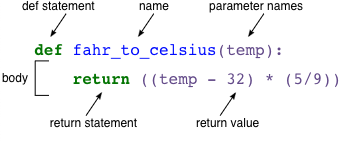
\includegraphics{assets/python-function.png}
\caption{The Blueprint for a Python Function}
\end{figure}

The function definition opens with the keyword \texttt{def} followed by
the name of the function (\texttt{fahr\_to\_celsius}) and a
parenthesized list of parameter names (\texttt{temp}). The body of the
function, the statements that are executed when it runs is indented
below the definition line. The body concludes with a \texttt{return}
keyword followed by the return value.

When we call the function, the values we pass to it are assigned to
those variables so that we can use them inside the function. Inside the
function, we use a return statement to send a result back to whoever
asked for it.

Let's try running our function.

\begin{Shaded}
\begin{Highlighting}[]
\NormalTok{fahr_to_celsius(}\DecValTok{32}\NormalTok{)}
\end{Highlighting}
\end{Shaded}

This command should call our function, using ``32'' as the input and
return the function value.

In fact, calling our own function is no different from calling any other
function:

\begin{Shaded}
\begin{Highlighting}[]
\BuiltInTok{print}\NormalTok{(}\StringTok{'freezing point of water:'}\NormalTok{, fahr_to_celsius(}\DecValTok{32}\NormalTok{), }\StringTok{'C'}\NormalTok{)}
\end{Highlighting}
\end{Shaded}

\begin{verbatim}
## freezing point of water: 0.0 C
\end{verbatim}

\begin{Shaded}
\begin{Highlighting}[]
\BuiltInTok{print}\NormalTok{(}\StringTok{'boiling point of water:'}\NormalTok{, fahr_to_celsius(}\DecValTok{212}\NormalTok{), }\StringTok{'C'}\NormalTok{)}
\end{Highlighting}
\end{Shaded}

\begin{verbatim}
## boiling point of water: 100.0 C
\end{verbatim}

We've successfully called the function that we defined, and we have
access to the value that we returned.

\hypertarget{composing-functions}{%
\section{Composing Functions}\label{composing-functions}}

Now that we've seen how to turn Fahrenheit into Celsius, we can also
write the function to turn Celsius into Kelvin:

\begin{Shaded}
\begin{Highlighting}[]
\KeywordTok{def}\NormalTok{ celsius_to_kelvin(temp_c):}
    \ControlFlowTok{return}\NormalTok{ temp_c }\OperatorTok{+} \FloatTok{273.15}
\BuiltInTok{print}\NormalTok{(}\StringTok{'freezing point of water in Kelvin:'}\NormalTok{, celsius_to_kelvin(}\FloatTok{0.}\NormalTok{))}
\end{Highlighting}
\end{Shaded}

\begin{verbatim}
## freezing point of water in Kelvin: 273.15
\end{verbatim}

What about converting Fahrenheit to Kelvin? We could write out the
formula, but we don't need to. Instead, we can compose the two functions
we have already created:

\begin{Shaded}
\begin{Highlighting}[]
\KeywordTok{def}\NormalTok{ fahr_to_kelvin(temp_f):}
\NormalTok{    temp_c }\OperatorTok{=}\NormalTok{ fahr_to_celsius(temp_f)}
\NormalTok{    temp_k }\OperatorTok{=}\NormalTok{ celsius_to_kelvin(temp_c)}
    \ControlFlowTok{return}\NormalTok{ temp_k}
\BuiltInTok{print}\NormalTok{(}\StringTok{'boiling point of water in Kelvin:'}\NormalTok{, fahr_to_kelvin(}\FloatTok{212.0}\NormalTok{))}
\end{Highlighting}
\end{Shaded}

\begin{verbatim}
## boiling point of water in Kelvin: 373.15
\end{verbatim}

This is our first taste of how larger programs are built, we define
basic operations, then combine them in ever-large chunks to get the
effect we want.

\hypertarget{variables-inside-and-outside-functions}{%
\section{Variables Inside and Outside
Functions}\label{variables-inside-and-outside-functions}}

The function is insulated from the rest of the program. Things that
happen in there don't affect what goes on elsewhere. Meaning we can
re-use variable names inside the function that we used elsewhere without
polluting them. Look what happens when the following piece of code is
run

\begin{Shaded}
\begin{Highlighting}[]
\NormalTok{f }\OperatorTok{=} \DecValTok{0}
\NormalTok{k }\OperatorTok{=} \DecValTok{0}
\KeywordTok{def}\NormalTok{ f2k(f):}
\NormalTok{    k }\OperatorTok{=}\NormalTok{ ((f}\DecValTok{-32}\NormalTok{)}\OperatorTok{*}\NormalTok{(}\FloatTok{5.0}\OperatorTok{/}\FloatTok{9.0}\NormalTok{)) }\OperatorTok{+} \FloatTok{273.15}
    \ControlFlowTok{return}\NormalTok{ k}
\BuiltInTok{print}\NormalTok{( f2k(}\DecValTok{8}\NormalTok{) )}
\BuiltInTok{print}\NormalTok{( f2k(}\DecValTok{41}\NormalTok{) )}
\BuiltInTok{print}\NormalTok{( f2k(}\DecValTok{32}\NormalTok{) )}
\BuiltInTok{print}\NormalTok{(k)}
\end{Highlighting}
\end{Shaded}

\begin{Shaded}
\begin{Highlighting}[]
\FloatTok{259.81666666666666}
\FloatTok{287.15}
\FloatTok{273.15}
\DecValTok{0}
\end{Highlighting}
\end{Shaded}

\texttt{k} is 0 because the \texttt{k} inside the function \texttt{f2k}
doesn't know about the \texttt{k} defined outside the function.

\hypertarget{quiz-4}{%
\section{Quiz}\label{quiz-4}}

\begin{enumerate}
\def\labelenumi{\arabic{enumi}.}
\tightlist
\item
  ``Adding'' two strings produces their concatenation
  \texttt{\textquotesingle{}a\textquotesingle{}\ +\ \textquotesingle{}b\textquotesingle{}}
  is \texttt{\textquotesingle{}ab\textquotesingle{}}. Write a function
  called \texttt{fence} that takes two parameters called
  \texttt{original} and \texttt{wrapper} and returns a new string that
  has the wrapper character at the beginning and end of the original. A
  call to your function should look like this:
\end{enumerate}

\begin{Shaded}
\begin{Highlighting}[]
\BuiltInTok{print}\NormalTok{(fence(}\StringTok{'name'}\NormalTok{, }\StringTok{'*'}\NormalTok{))}
\end{Highlighting}
\end{Shaded}

\begin{enumerate}
\def\labelenumi{\arabic{enumi}.}
\setcounter{enumi}{1}
\tightlist
\item
  Note that \texttt{return} and \texttt{print} are not
  interchangeable.\texttt{print} is a Python function that \emph{prints}
  data to the screen. It enables us, \emph{users}, see the data.
  \texttt{return} statement, on the other hand, makes data visible to
  the program.
\end{enumerate}

Let's have a look at the following function:

\begin{Shaded}
\begin{Highlighting}[]
\KeywordTok{def}\NormalTok{ add(a, b):}
   \BuiltInTok{print}\NormalTok{(a }\OperatorTok{+}\NormalTok{ b)}
\end{Highlighting}
\end{Shaded}

What will we see if we execute the following commands?

\begin{Shaded}
\begin{Highlighting}[]
\NormalTok{A }\OperatorTok{=}\NormalTok{ add(}\DecValTok{7}\NormalTok{, }\DecValTok{3}\NormalTok{)}
\BuiltInTok{print}\NormalTok{(A)}
\end{Highlighting}
\end{Shaded}

\begin{enumerate}
\def\labelenumi{\arabic{enumi}.}
\setcounter{enumi}{2}
\tightlist
\item
  If the variable \texttt{s} refers to a string, then \texttt{s{[}0{]}}
  is the string's first character and \texttt{s{[}-1{]}} is its last.
  Write a function called \texttt{outer} that returns a string made up
  of just the first and last characters of its input. A call to your
  function should look like this:
\end{enumerate}

\begin{Shaded}
\begin{Highlighting}[]
\BuiltInTok{print}\NormalTok{(outer(}\StringTok{'helium'}\NormalTok{))}
\end{Highlighting}
\end{Shaded}

\begin{enumerate}
\def\labelenumi{\arabic{enumi}.}
\setcounter{enumi}{3}
\tightlist
\item
  Rescaling an Array
\end{enumerate}

Write a function \texttt{rescale} that takes a list as input and returns
a corresponding list of values scaled to lie in the range 0.0 to 1.0.

(Hint: If \texttt{L} and \texttt{H} are the lowest and highest values in
the original array, then the replacement for a value \texttt{v} should
be \texttt{(v-L)\ /\ (H-L)}. The \texttt{max()} function returns the
biggest value in a list)

\begin{enumerate}
\def\labelenumi{\arabic{enumi}.}
\setcounter{enumi}{4}
\tightlist
\item
  Consider this code:
\end{enumerate}

\begin{Shaded}
\begin{Highlighting}[]
\NormalTok{a }\OperatorTok{=} \DecValTok{3}
\NormalTok{b }\OperatorTok{=} \DecValTok{7}
\KeywordTok{def}\NormalTok{ swap(a, b):}
\NormalTok{    temp }\OperatorTok{=}\NormalTok{ a}
\NormalTok{    a }\OperatorTok{=}\NormalTok{ b}
\NormalTok{    b }\OperatorTok{=}\NormalTok{ temp}
\NormalTok{swap(a, b)}
\BuiltInTok{print}\NormalTok{(a, b)}
\end{Highlighting}
\end{Shaded}

Which of the following would be printed if you were to run this code?
Why did you pick this answer?

\begin{enumerate}
\def\labelenumi{\arabic{enumi}.}
\tightlist
\item
  \texttt{7\ 3}
\item
  \texttt{3\ 7}
\item
  \texttt{3\ 3}
\item
  \texttt{7\ 7}
\end{enumerate}

\hypertarget{using-packages}{%
\chapter{Using Packages}\label{using-packages}}

Packages are an important part of the Python `eco-system' that let us
use a wide variety of code written by other people. Good packages
provide functions, objects and methods that make working in a particular
problem domain a lot easier.

\hypertarget{using-and-installing-packages.}{%
\section{Using and Installing
Packages.}\label{using-and-installing-packages.}}

We've already seen how to load in packages using the \texttt{import}
statement. Here we load the \texttt{sys} package which has methods for
working with the underlying system - the \texttt{platform} is the name
of the operating system this code is running on.

\begin{Shaded}
\begin{Highlighting}[]
\ImportTok{import}\NormalTok{ sys}
\BuiltInTok{print}\NormalTok{( sys.platform )}
\end{Highlighting}
\end{Shaded}

\begin{verbatim}
## darwin
\end{verbatim}

Some packages come as standard when Python is installed, some come from
external sources and must be installed individually. There are multiple
methods of installing packages. Assuming you set up Python using
Anaconda for this book then you can use \texttt{conda} itself. Another
more general way of installing packages is from PyPI, the Python Package
Index.

None of these are done from within Python itself, and must be done from
the regular command-line. The general form is:

\begin{Shaded}
\begin{Highlighting}[]
\ExtensionTok{conda}\NormalTok{ install package_name}
\ExtensionTok{pip}\NormalTok{ install package_name}
\end{Highlighting}
\end{Shaded}

\hypertarget{the-pyvcf-package}{%
\section{The PyVCF Package}\label{the-pyvcf-package}}

VCF files (variant call format) are files that describe SNPs and small
indels in alignments from high-throughput sequencing data. The
\texttt{PyVCF} package provides a lot of functionality for working with
such files and the record they contain.

\hypertarget{vcf-files---a-brief-introduction}{%
\subsection{VCF files - a brief
introduction}\label{vcf-files---a-brief-introduction}}

A VCF file is a column format file where each row represents a SNP/Indel
record and the columns represent the variables of things like
Chromosome, Position, Reference Genome Allele, Alternative Genome Allele
etc. Here's what one record looks like.

\begin{longtable}[]{@{}ccccccc@{}}
\caption{Table continues below}\tabularnewline
\toprule
\begin{minipage}[b]{0.09\columnwidth}\centering
CHROM\strut
\end{minipage} & \begin{minipage}[b]{0.09\columnwidth}\centering
POS\strut
\end{minipage} & \begin{minipage}[b]{0.13\columnwidth}\centering
ID\strut
\end{minipage} & \begin{minipage}[b]{0.07\columnwidth}\centering
REF\strut
\end{minipage} & \begin{minipage}[b]{0.07\columnwidth}\centering
ALT\strut
\end{minipage} & \begin{minipage}[b]{0.08\columnwidth}\centering
QUAL\strut
\end{minipage} & \begin{minipage}[b]{0.10\columnwidth}\centering
FILTER\strut
\end{minipage}\tabularnewline
\midrule
\endfirsthead
\toprule
\begin{minipage}[b]{0.09\columnwidth}\centering
CHROM\strut
\end{minipage} & \begin{minipage}[b]{0.09\columnwidth}\centering
POS\strut
\end{minipage} & \begin{minipage}[b]{0.13\columnwidth}\centering
ID\strut
\end{minipage} & \begin{minipage}[b]{0.07\columnwidth}\centering
REF\strut
\end{minipage} & \begin{minipage}[b]{0.07\columnwidth}\centering
ALT\strut
\end{minipage} & \begin{minipage}[b]{0.08\columnwidth}\centering
QUAL\strut
\end{minipage} & \begin{minipage}[b]{0.10\columnwidth}\centering
FILTER\strut
\end{minipage}\tabularnewline
\midrule
\endhead
\begin{minipage}[t]{0.09\columnwidth}\centering
20\strut
\end{minipage} & \begin{minipage}[t]{0.09\columnwidth}\centering
14370\strut
\end{minipage} & \begin{minipage}[t]{0.13\columnwidth}\centering
rs6054257\strut
\end{minipage} & \begin{minipage}[t]{0.07\columnwidth}\centering
G\strut
\end{minipage} & \begin{minipage}[t]{0.07\columnwidth}\centering
A\strut
\end{minipage} & \begin{minipage}[t]{0.08\columnwidth}\centering
29\strut
\end{minipage} & \begin{minipage}[t]{0.10\columnwidth}\centering
PASS\strut
\end{minipage}\tabularnewline
\bottomrule
\end{longtable}

\begin{longtable}[]{@{}cccc@{}}
\caption{Table continues below}\tabularnewline
\toprule
\begin{minipage}[b]{0.31\columnwidth}\centering
INFO\strut
\end{minipage} & \begin{minipage}[b]{0.17\columnwidth}\centering
FORMAT\strut
\end{minipage} & \begin{minipage}[b]{0.20\columnwidth}\centering
NA00001\strut
\end{minipage} & \begin{minipage}[b]{0.20\columnwidth}\centering
NA00002\strut
\end{minipage}\tabularnewline
\midrule
\endfirsthead
\toprule
\begin{minipage}[b]{0.31\columnwidth}\centering
INFO\strut
\end{minipage} & \begin{minipage}[b]{0.17\columnwidth}\centering
FORMAT\strut
\end{minipage} & \begin{minipage}[b]{0.20\columnwidth}\centering
NA00001\strut
\end{minipage} & \begin{minipage}[b]{0.20\columnwidth}\centering
NA00002\strut
\end{minipage}\tabularnewline
\midrule
\endhead
\begin{minipage}[t]{0.31\columnwidth}\centering
NS=3;DP=14;AF=0.5;DB;H2\strut
\end{minipage} & \begin{minipage}[t]{0.17\columnwidth}\centering
GT:GQ:DP:HQ\strut
\end{minipage} & \begin{minipage}[t]{0.20\columnwidth}\centering
0\textbar{}0:48:1:51,51\strut
\end{minipage} & \begin{minipage}[t]{0.20\columnwidth}\centering
1\textbar{}0:48:8:51,51\strut
\end{minipage}\tabularnewline
\bottomrule
\end{longtable}

\begin{longtable}[]{@{}c@{}}
\toprule
\begin{minipage}[b]{0.20\columnwidth}\centering
NA00003\strut
\end{minipage}\tabularnewline
\midrule
\endhead
\begin{minipage}[t]{0.20\columnwidth}\centering
1/1:43:5:.,.\strut
\end{minipage}\tabularnewline
\bottomrule
\end{longtable}

There's a lot of information in that one record, and each file has many
tens of thousands of records! !e wouldn't want to try and process tens
of thousands manually. Let's look at loading in a file and looping
through each record using the \texttt{PyVCF} package.

We've already seen that packages have functions we can call, and that
doing so can sometimes return objects of new types. We'll use that
pattern now to start processing a VCF file.

\hypertarget{the-vcf.reader-object}{%
\subsection{\texorpdfstring{The \texttt{vcf.Reader}
object}{The vcf.Reader object}}\label{the-vcf.reader-object}}

The first package function we'll need to use is \texttt{vcf.Reader}
which opens and connects to a file but doesn't do anything with it. It
gives us a reader object we can use to access the file. We just need the
file name that we wish to open.

\begin{Shaded}
\begin{Highlighting}[]
\ImportTok{import}\NormalTok{ vcf}
\NormalTok{vcf_reader }\OperatorTok{=}\NormalTok{ vcf.Reader(}\BuiltInTok{open}\NormalTok{(}\StringTok{'/Users/macleand/Desktop/example.vcf'}\NormalTok{, }\StringTok{'r'}\NormalTok{))}
\end{Highlighting}
\end{Shaded}

Now we can go ahead and extract the VCF records by using the reader
object we created in a loop

\begin{Shaded}
\begin{Highlighting}[]
\ControlFlowTok{for}\NormalTok{ record }\KeywordTok{in}\NormalTok{ vcf_reader:}
  \BuiltInTok{print}\NormalTok{( record )}
  \BuiltInTok{print}\NormalTok{(}\BuiltInTok{type}\NormalTok{(record))}
\end{Highlighting}
\end{Shaded}

\begin{verbatim}
## Record(CHROM=20, POS=14370, REF=G, ALT=[A])
## <class 'vcf.model._Record'>
## Record(CHROM=20, POS=17330, REF=T, ALT=[A])
## <class 'vcf.model._Record'>
## Record(CHROM=20, POS=1110696, REF=A, ALT=[G, T])
## <class 'vcf.model._Record'>
## Record(CHROM=20, POS=1230237, REF=T, ALT=[None])
## <class 'vcf.model._Record'>
## Record(CHROM=20, POS=1234567, REF=GTCT, ALT=[G, GTACT])
## <class 'vcf.model._Record'>
\end{verbatim}

This does the code loop for every record in the file.

\hypertarget{the-vcf.record-object}{%
\subsection{\texorpdfstring{The \texttt{vcf.Record}
object}{The vcf.Record object}}\label{the-vcf.record-object}}

Every time we loop we get a new \texttt{vcf.Record} object. This is a
special sort of object provided by the \texttt{PyVCF} package that
represents the VCF record. We already saw how objects have methods -
special functions that apply straight to the data in that object.
\texttt{PyVCF} is no exception. As well as methods, objects can have
properties called attributes.

\hypertarget{object-attributes}{%
\subsection{Object Attributes}\label{object-attributes}}

Attributes of an object are different from functions of an object in
that they tend to be things that just are rather than things that are
computed. So a hypothetical \texttt{shape} object representing a
geometric shape might have an attribute called \texttt{sides}. This
wouldn't need recomputing as it would be the same everytime.

Attributes are easy to spot as they use the \texttt{object} dot
\texttt{.} syntax, omitting the brackets at the end of the attribute
name. Let's examine that using the \texttt{.POS} attribute.

\begin{Shaded}
\begin{Highlighting}[]
\NormalTok{vcf_reader }\OperatorTok{=}\NormalTok{ vcf.Reader(}\BuiltInTok{open}\NormalTok{(}\StringTok{'/Users/macleand/Desktop/example.vcf'}\NormalTok{, }\StringTok{'r'}\NormalTok{))}
\ControlFlowTok{for}\NormalTok{ record }\KeywordTok{in}\NormalTok{ vcf_reader:}
  \BuiltInTok{print}\NormalTok{( record.POS )}
\end{Highlighting}
\end{Shaded}

\begin{verbatim}
## 14370
## 17330
## 1110696
## 1230237
## 1234567
\end{verbatim}

Here we can see that we get the position of each SNP/Indel in the
chromosome from \texttt{.POS}. Note that we had to redo the vcf\_reader
creation - this is because the \texttt{vcf.Reader} object has in a sense
``got to the end'' of the data the first time we used it. It needs
re-winding to the start and one way to do that is to recreate it and
thereby reset it.

\hypertarget{finding-the-methods-and-attributes-an-object-has}{%
\subsubsection{Finding the methods and attributes an object
has}\label{finding-the-methods-and-attributes-an-object-has}}

If we want to find out what methods or attributes an object has we can
use the \texttt{dir()} function which gives us these for an object.

\begin{Shaded}
\begin{Highlighting}[]
\BuiltInTok{print}\NormalTok{( }\BuiltInTok{dir}\NormalTok{(vcf_reader) )}
\end{Highlighting}
\end{Shaded}

\begin{verbatim}
## ['__class__', '__delattr__', '__dict__', '__dir__', '__doc__', '__eq__', '__format__', '__ge__', '__getattribute__', '__gt__', '__hash__', '__init__', '__init_subclass__', '__iter__', '__le__', '__lt__', '__module__', '__ne__', '__new__', '__next__', '__reduce__', '__reduce_ex__', '__repr__', '__setattr__', '__sizeof__', '__str__', '__subclasshook__', '__weakref__', '_alt_pattern', '_column_headers', '_format_cache', '_header_lines', '_map', '_parse_alt', '_parse_info', '_parse_metainfo', '_parse_sample_format', '_parse_samples', '_prepend_chr', '_reader', '_row_pattern', '_sample_indexes', '_separator', '_tabix', 'alts', 'contigs', 'encoding', 'fetch', 'filename', 'filters', 'formats', 'infos', 'metadata', 'reader', 'samples']
\end{verbatim}

So the list is really large! Some methods and attributes begin with
\texttt{\_} underscore characters. By convention these are things that
are used internally by the object - so you don't need to worry about
those. We can filter the ones we can use, by building a list of ones
that \emph{don't} start with '\_'

\begin{Shaded}
\begin{Highlighting}[]
\NormalTok{attrs }\OperatorTok{=} \BuiltInTok{dir}\NormalTok{(vcf_reader)}
\NormalTok{keepers }\OperatorTok{=}\NormalTok{ []}
\ControlFlowTok{for}\NormalTok{ a }\KeywordTok{in}\NormalTok{ attrs:}
  \ControlFlowTok{if} \KeywordTok{not}\NormalTok{ a.startswith(}\StringTok{"_"}\NormalTok{):}
\NormalTok{    keepers.append(a)}
\BuiltInTok{print}\NormalTok{( keepers )}
\end{Highlighting}
\end{Shaded}

\begin{verbatim}
## ['alts', 'contigs', 'encoding', 'fetch', 'filename', 'filters', 'formats', 'infos', 'metadata', 'reader', 'samples']
\end{verbatim}

This is a much shorter list. You can see the online documentation for
the object here
\href{}{https://pyvcf.readthedocs.io/en/latest/API.html\#vcf-reader}

Pretty much all objects and packages will have some online documentation
so you can \emph{usually} find something. Sometimes it's a bit sparse,
unfortunately.

\hypertarget{quiz-5}{%
\section{Quiz}\label{quiz-5}}

\begin{enumerate}
\def\labelenumi{\arabic{enumi}.}
\tightlist
\item
  Using \texttt{PyVCF}, calculate how many of the records are SNPs and
  how many are Indels. Use the documentation to see how you might
  achieve this -
  \href{}{https://pyvcf.readthedocs.io/en/latest/API.html\#vcf-model-record}
\item
  For each SNP, work out whether it's an A-G or C-T, a so-called
  transition. Would your method be efficient on a file of thousands of
  SNPS?
\item
  Which record has the greatest number of alleles? Would your method be
  efficient on a file of thousands of SNPs/Indels?
\item
  How many alternative alleles are heterozygous, for each record?
\end{enumerate}

\hypertarget{putting-code-into-scripts}{%
\chapter{Putting code into scripts}\label{putting-code-into-scripts}}

Scripts are files full of code that has been put together in order to do
a particular task. The idea being that the code will get re-run many
times and not just as a one off.

Building a script is usually pretty easy - just type the code in to a
text file.

You'll need a text editor, a program that deals with text but not in the
same way as a word processor. Many such programs are available, try the
options below

\begin{enumerate}
\def\labelenumi{\arabic{enumi}.}
\tightlist
\item
  TextMate (macOS) \href{}{https://macromates.com/}
\item
  Atom (macOS/Windows) \href{}{https://atom.io/}
\item
  Notepad++ (Windows) \href{}{https://notepad-plus-plus.org/}
\end{enumerate}

\hypertarget{the-script-header}{%
\section{The Script Header}\label{the-script-header}}

Most Python scripts have this on the first line

\begin{verbatim}
#!/usr/bin/env python
\end{verbatim}

This is a Unix/Linux convention that affects how those systems interpret
the file. Leave it in for convention's sake.

\hypertarget{the-filename-extension}{%
\section{The Filename Extension}\label{the-filename-extension}}

By convention, Python scripts end in the extension, \texttt{.py}.

So if we have the following in a file called \texttt{hello\_world.py},
we have a Python script.

\begin{verbatim}
#!/usr/bin/env python

print("Hello, World!")
\end{verbatim}

\hypertarget{running-a-python-script}{%
\section{Running a Python script}\label{running-a-python-script}}

Once created, the script itself is run from the \texttt{python} command
on the command line. \texttt{python} is just a regular program that
accepts a python script filename as its argument and runs the code in
the script.

Here's an example terminal session that runs a script.

\begin{verbatim}
Last login: Thu Dec  6 10:59:32 on ttys000
~/Desktop macleand$ python hello_world.py

Hello, World!

~/Desktop macleand$
\end{verbatim}

\hypertarget{getting-options-from-the-command-line}{%
\section{Getting Options from the Command
Line}\label{getting-options-from-the-command-line}}

A good reason for creating scripts is because you want to be able to
re-run the code in them. Sometimes you'll want to change some aspect or
behaviour of the code according to settings given on the command-line.
For example, you might want to work on a different input file each time.
We can access the text from the command-line in the script, using the
\texttt{sys.argv} attribute in the \texttt{sys} module.

Imagine the command line

\begin{verbatim}
python my_script.py OPTION_1 option_2
\end{verbatim}

We access it like this

\begin{Shaded}
\begin{Highlighting}[]
\CommentTok{#!/usr/bin/env python}
\ImportTok{import}\NormalTok{ sys}
\BuiltInTok{print}\NormalTok{( sys.argv )}
\end{Highlighting}
\end{Shaded}

\begin{verbatim}
['my_script.py', 'OPTION_1', 'option_2']
\end{verbatim}

The \texttt{sys.argv} attribute gives us a list of the command line
options. The first item in the list is the script name, the options come
after that. So we can access the options by indexing the
\texttt{sys.argv} list

\begin{verbatim}
python my_script.py OPTION_1 option_2
\end{verbatim}

\begin{Shaded}
\begin{Highlighting}[]
\CommentTok{#!/usr/bin/env python}
\ImportTok{import}\NormalTok{ sys}
\NormalTok{first_option }\OperatorTok{=}\NormalTok{ sys.argv[}\DecValTok{1}\NormalTok{]}
\NormalTok{second_option }\OperatorTok{=}\NormalTok{ sys.argv[}\DecValTok{2}\NormalTok{]}
\BuiltInTok{print}\NormalTok{(second_option, first_option)}
\end{Highlighting}
\end{Shaded}

\begin{verbatim}
option_2 OPTION_1
\end{verbatim}

\hypertarget{quiz-6}{%
\section{Quiz}\label{quiz-6}}

\begin{enumerate}
\def\labelenumi{\arabic{enumi}.}
\tightlist
\item
  Create a script that writes `Hello, World!' to the screen. Run it.
\item
  Create a script that takes one argument and prints that to the screen
  as \texttt{You\ said..\ \textless{}argument\textgreater{}} - replacing
  \texttt{\textless{}argument\textgreater{}} with the value you give on
  the command line.
\item
  Create a script that takes two numbers from the command line and adds
  them together and prints the result.
\end{enumerate}

\hypertarget{putting-it-all-together}{%
\chapter{Putting It All Together}\label{putting-it-all-together}}

\hypertarget{a-challenge-in-python}{%
\section{A Challenge in Python}\label{a-challenge-in-python}}

This file
\href{}{ftp://ftp.sra.ebi.ac.uk/vol1/fastq/SRR020/SRR020192/SRR020192.fastq.gz}
contains next generation sequencing reads in \texttt{fastq} format.

Write a Python script that use the BioPython package to

\begin{enumerate}
\def\labelenumi{\arabic{enumi}.}
\tightlist
\item
  Count the reads in the \texttt{fastq} file
\item
  Filter out low-quality reads from the \texttt{fastq} file
\item
  Calculate how many reads are retained
\item
  Use at least one user-defined function
\end{enumerate}

Acknowledgements

Some of the quizzes and examples in this book particularly those in
Chapters 3 to 7 are taken from the Software Carpentry lesson on
Programming in Python
\href{}{http://swcarpentry.github.io/python-novice-inflammation/}. Other
examples in Chapter 9 and 10 are taken from the Biopython tutorial
\href{}{http://biopython.org/DIST/docs/tutorial/Tutorial.html} and the
PyVCF tutorial \href{}{https://pyvcf.readthedocs.io/}.These are re-used
under their respective licences.

The rest of the materials are licensed under Creative Commons 0.

\bibliography{book.bib,packages.bib}


\end{document}
